\chapter{Practical Appliance}
As described in the previous chapter, this one will walk through the requirement engineering process for a B2B marketing application. A label based on a capital letter and a hierarchical number will be used for itemized \mbox{information (\textbf{I})}, \mbox{functional requirements (\textbf{FR})} and \mbox{quality requirements (\textbf{QR})} (e.g. \ssay{\textbf{I3.2.3}}).
\section{Input information}
\subsection{The Sponsor}
The sponsor, he explained, that he would like to have an application or website, which he can give to a customer to play around with and to get to know the skills of IBM \parencite{Sachs.20.04.2017}. As a legacy from times when IBM was mainly a mainframe hardware supplier, IBM is perceived with its past skill , he further points out \parencite{Sachs.20.04.2017}. Therefore the app must arouse the interest of the potential customer and display that IBM has experience, knowledge and skills in the domain of banking software migration. 

\paragraph{} As a condition for access by the potential customer, the sponsor required some kind of authentication, which would lock the customer out after two weeks time, if the access is not extended by an IBM opportunity owner\parencite[cf.][]{Sachs.2017}.

\paragraph{} 'Opportunity owner' in this thesis refers to the responsible employee for a opportunity to sell IBM services.

\paragraph{} As a visual appearance, the sponsor demanded a stereotypical generalized online banking application \parencite[cf.][]{Sachs.2017}.

\paragraph{} Constraining the development of the application, the sponsor requested that the application will not generate costs when not in use, is developed by corporate student in their three month practical - as it is common at IBM - and will be developed in iterative development cycles \parencite[cf.][]{Sachs.2017}. This approach is requested to ensure usable products after the three month term.

\paragraph{} Summarized:

\begin{closeItem}
    \item [\textbf{I1}] When a customer uses the application, the system shall provide him with the ability to receive information about IBM skills.
    \item [\textbf{I2}] When a customer tries to use the site, the system shall request some kind of authentication.
    \item [\textbf{I2.1}] When customer access rights age two weeks without being extended, the system shall revoke the access rights.
    \item [\textbf{I2.2}\label{R2.2}] When a user is an opportunity owner of IBM the application, the system shall provide the user with the ability to extend customer access rights.
    \item [\textbf{I3}] The system shall superficially appear like a mobile online banking application.
\end{closeItem}

\paragraph{} It is implied by \textbf{I2.2}, that IBM opportunity owner must be able to log into the system in a way that proves their employment status at IBM. This causes a new Requirement:

\begin{closeItem}
    \item [\textbf{I4}] When the system is accessed, it shall provide IBM opportunity owners the ability to log in with their corporate identity.
\end{closeItem}

\subsection{Organizational Standards}
Subsequent to \textbf{I4}, IBM has a organizational standard for authentication on application, which are also available online: the so-called w3ID-Log in \parencite[cf.][]{IBMCorporation.2016}.

\begin{closeItem}
    \item [\textbf{I4.1}] When a user wants to identify as an IBM opportunity owner, the system shall utilize w3ID for authentication.
\end{closeItem}

\paragraph{} In addition to authentication procedures, IBM requires all applications to follow a set of rules:

\paragraph{} The development must follow the 'MobileFirst'-idea, if applicable \parencite[cf.][]{IBMCorporation.2016}. This is explained as acting on the principle to develop everything for mobile devices first. That of course only applies only on applications intended for use on mobile devices.

\paragraph{} Mobile device referees to small screen devices with no keyboard in this context \parencite[cf.][]{Duong.2014}. Afterwards the design and functionality may be extended to larger devices with more peripheral devices (mouse, keyboard, etc.) and larger screens.

\paragraph{} The application, to this point, do not show any reason to not be available on mobile device, therefore:

\begin{closeItem}
    \item [\textbf{I5}] When a developer does work for the system, the developer should do the work for mobile devices prioritized.
\end{closeItem}

\subsection{Regulations}
No proof could be found for any regulation concerning the functionality of the application. To this point, it will not collect any information, display any personal information, export US-American intellectual property or show any other regulation related behaviour. On the other hand, this research must be done exhaustively by a legal expert, which was not available for this research.

\subsection{Domain Information}
The domain of B2B marketing is described in \Cref{ssec:b2b} on \cpagerefrange{ssec:b2b}{endb2b}. Important conclusions are: 

\begin{closeItem}
    \item [\textbf{I6}] When creating the stakeholder map, the requirements engineer shall integrate the customer's stakeholders.
    \item [\textbf{I7}] When a B2B customer is approached, the communication should address to his or her individual case.
\end{closeItem}

Since the principle of attention economy suggests that attention of users may be lost quickly due to other factors (cf. \Cref{ssec:attention}):

\begin{closeItem}
    \item [\textbf{I8}] When a customer stops using the application, the application should be able to retrieve back his or her attention.
\end{closeItem}

\paragraph{}

\subsection{Stakeholder Needs}
As described earlier, in order to identify stakeholder need, the stakeholders must be identified. Firstly, all stakeholder which were directly mentioned to this point can be identified:

\begin{closeItemCol}
    \item customer (\textbf{I1})
    \item sponsor
    \item IBM opportunity owner (\textbf{I2.2})
    \item IBM Corporation
    \item developer (\textbf{I5})
\end{closeItemCol}

The sponsor and IBM corporation are not tracked back, since they are the basic setting for the research.

\paragraph{} These stakeholders are pretty vague. Who is the \ssay{customer}. Deriving from the sponsors information, that the application should be handed to the customer during a bidding procedure as result of a call for proposal, the author deduces based on past experience that the \ssay{customer} can either be the procurement of the calling company, the future steering committee of the to-be project naming the management of the demanding company. 

\paragraph{} This leads to the \ssay{customer} to be subdivided. The sponsor, the opportunity owner and the contributor can all be classified as IBM employee.

\begin{closeItemCol}
    \item customer (\textbf{I1})
    \begin{itemize}
        \item procurement officer
        \item operational manager
        \item IT department representative
        \item legal and compliance advisor
        \item finance representative
    \end{itemize} \columnbreak
    
    \item IBM employee 
    \begin{itemize}
        \item sponsor
        \item developer (\textbf{I5})
        \item opportunity owner (\textbf{I2.2})
    \end{itemize}
    \item IBM Corporation
\end{closeItemCol}

In reference to the specialties of B2B marketing mentioned on \cpageref{ssec:b2b}, the customer demand for service is only derived from their customer demands. Therefore, these customers have to be included as well. 

\paragraph{} Basically, those can be separated into consumers and other businesses. As of the explanation from the sponsor, the consumer group is split into 2 groups: core banking customer, meaning people who only have bank account and credits, and those who additionally do stock broking. 

\paragraph{} Same is somehow true for B2B clients, but those are much more diverse than consumers. They may have individual terms and conditions, distribute stocks and so on. 

\paragraph{} For simplicity, we regard consumers and companies as equal as long as the diversity does not have an impact.

\paragraph{}
Regarding the professional context of a bank, it becomes clear that two of their stakeholder are of special importance: Firstly, the stock brokers require tax statements by the bank, which are critical for the banks clients annual tax declaration. Secondly, the \ssay{Bundesanstalt für 
Finanzdienstleistungsaufsicht} (BaFin), the German institute for financial supervision, requires notes on a regular basis from the bank.

\begin{closeItem}
    \item [\textbf{I9}] When information is collected for the application, the creators should not forget the regular notes to the BaFin.
    \item [\textbf{I10}] When information is collected for the application, the creators should not forget about stock trading tax issues.
\end{closeItem}

\vspace{2em}


\begin{closeItemCol}
    \NoIndent{\textbf{IBM's stakeholders:}}
    \item customer (\textbf{I1})
    \begin{itemize}
        \item procurement officer
        \item operational manager
        \item IT department representative
        \item legal and compliance advisor
        \item finance representative
    \end{itemize}
    \item IBM employee 
    \begin{itemize}
        \item sponsor
        \item developer (\textbf{I5})
        \item opportunity owner (\textbf{I2.2})
    \end{itemize}
    \item IBM Corporation
    \columnbreak
    \NoIndent{\textbf{Stakeholders of the customer:}}
    \item BaFin
    \item stock broker
    \item core banking customers
\end{closeItemCol}

\subsubsection{Stakeholder Maps}
For translation into stakeholder maps as described in \Cref{ssec:personas}, the stakeholders must be ordered by intensity of usage, and by influence on the service. Each from the perspective of the service. Therefore the stakeholders of IBM will be ordered by the usage and influence of the desired marketing app, and the customer's stakeholders by the usage of and influence on the banking service.

\paragraph{}
Ordering the IBM's stakeholders by usage is pretty straight foreword: The IBM opportunity owners will be the most frequent users, because they will use the application frequently to allow customer access. All customer roles will be using the application for a single approximately two week time period what makes them irregular users.
The developer and IBM Corporation will not be users of the application, one only accessing the application for test reasons, the other executing only regulatory authority. 

\paragraph{} More carefully, the order of influence must be generated, since the term influence can be ambiguous: On the one hand, it could mean the influence on the app development - which is the correct interpretation (cf. \cpageref{fig:stakeMap}) -, on the other hand, the influence on the buying decision of the customer might be of interest.


\begin{figure}[H]
    \centering
    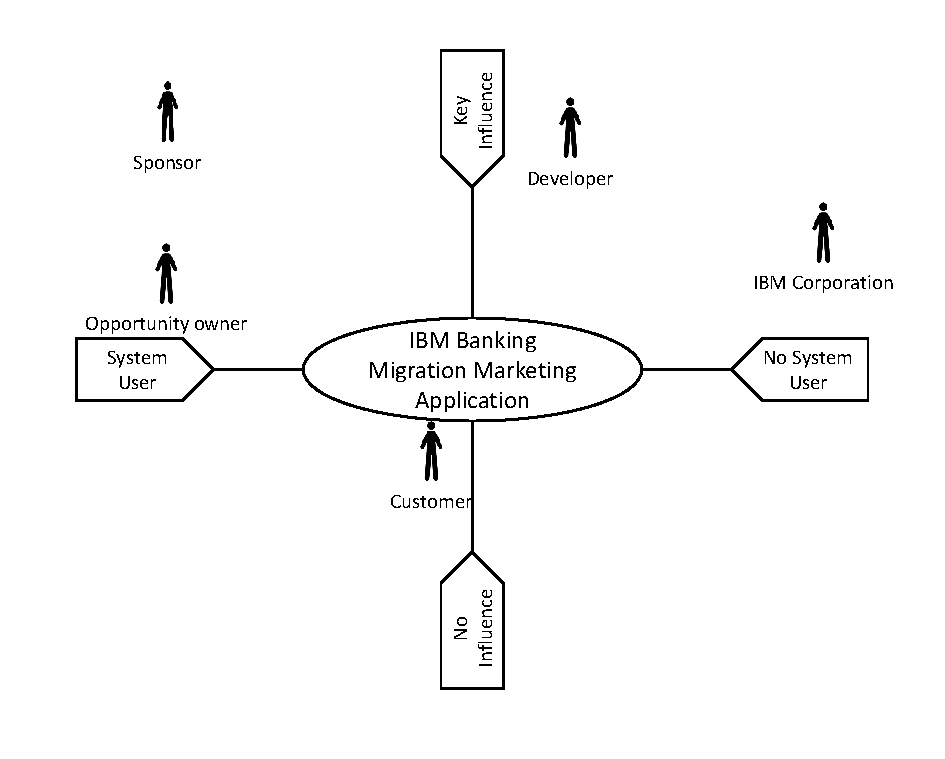
\includegraphics[height=.5\textheight]{img/smMarketingApp.pdf}
    \caption[Stakeholder Map of IBM Marketing Application]{Stakeholder Map of IBM Marketing Application (own illustration)}
    \label{fig:smIBM}
\end{figure}

As to be seen in \Cref{fig:smIBM} the order in influence was decided to be in the following order: The sponsor being most influential, since he is supervising the application life cycle from the conception via development to deployment and can empower influence at any time. Secondly, the developer has got great impact on the application, because his skills and commitment shape the application. Thirdly, the IBM Cooperation influences the application by requiring certain development and style guidelines. At fourth position come the opportunity owner, which do not directly influence the application, but may supply feedback or ideas during the development process. Least influential are the customer employees deciding over the purchase. They have no impact what so ever over the application. 

\paragraph{} Regarding the customer's needs and pain points, a look at their stakeholder map can be taken:

\begin{figure}[H]
    \centering
    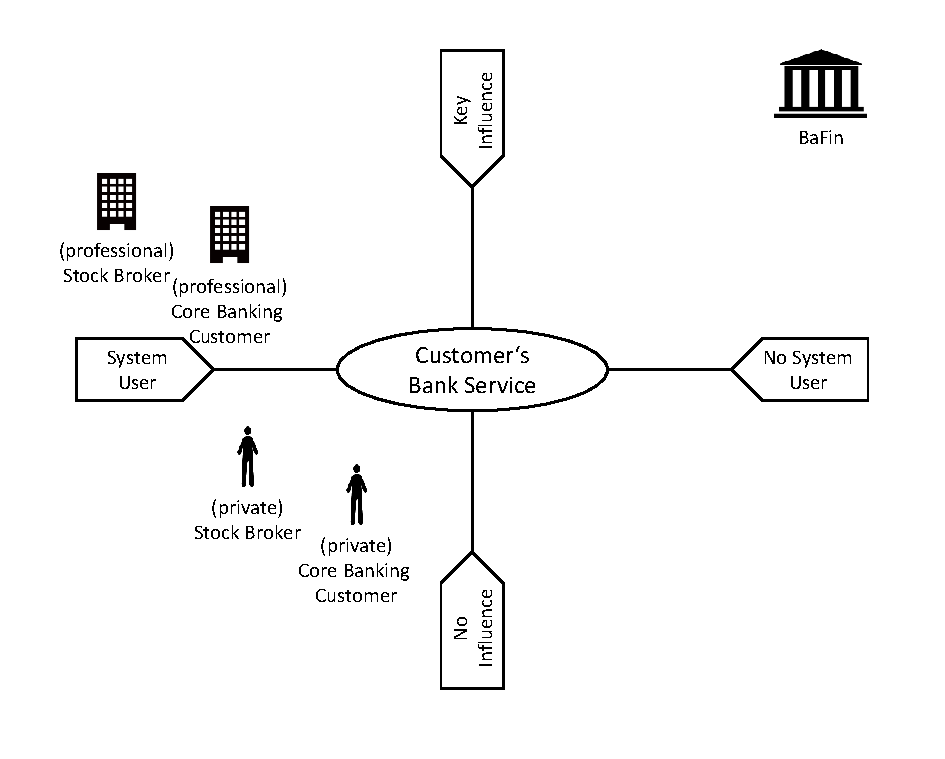
\includegraphics[height=.5\textheight]{img/smBank.pdf}
    \caption[Curate Bank Stakeholder Map]{Curate Bank Stakeholder Map (own illustration)}
    \label{fig:my_label}
\end{figure}

Regarded most influential, the BaFin is not using the banking service. This is certainly false for at least one bank since they have to transfer money as well as any other entity of the market. On the other hand, the BaFin will most certainly not have bank accounts at a major part of the banks operating in Germany. Second most influential are B2B stock trading customers. B2B customer do have more individual terms and conditions with the banks and can thereby make a huger impact on the bank's services. Stock trading customers do have a higher influence level due to the broader interaction with the bank. Therefore, the private customers rank fourth (stock trading) and fifth (core banking only).

\paragraph{} In terms of usage, stock brokers will be most likely to use the banking service more often, because they have more to do. Professionals will use the bank service more frequently than private individuals, because most companies turn over more money than companies. 

\subsubsection{Personas}
The complete set of personas can be seen in the appendix (cf. \cpagerefrange{persbegin}{persend}). As an exemplary case, follows the persona of Patrick Maurer (cf. \Cref{fig:PatrickMaurer}), who is a procurement manager at a bank in Frankfurt. He is kind of a diligent and wary once it comes to marketing presentations. This is because as a procurement manager, he is being held responsible, if what he ordered was not what it promised to be. 

\begin{figure}[H]
    \centering
    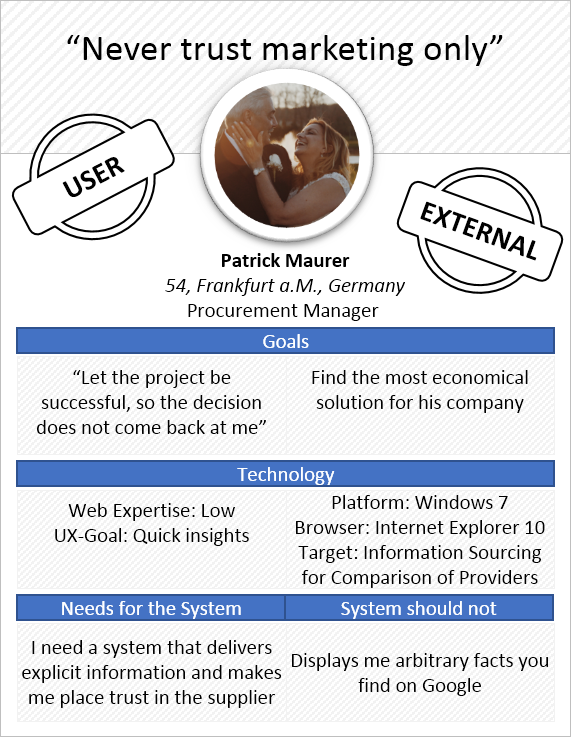
\includegraphics[height=.5\textheight]{img/diagrams/personas/customer1.png}
    \caption[Persona of Patrick Maurer]{Persona of Patrick Maurer (own illustration)}
    \label{fig:PatrickMaurer}
\end{figure}

He would use the application, if it gave him quick insights into the suppliers skills. What he refuses to take a look into are marketing phrases, which contain no controllable information or arbitrary facts, anyone can find out without deeper knowledge of the banking industry. As requirements for the system, he uses a PC running Windows 7 for work and browses the web with the pre-installed Internet Explorer. Since his company checks every Update by Microsoft for Bug before delivering them to the employees, he is sometimes not on the newest Version of the Software. He does not use a smart phone, but a classic cellphone.

\paragraph{}
The personal traits were results of past experience of the author. The reasons Patrick gained the technical traits, was to fulfill the overall statistics, as follows:
\begin{enumerate}
    \item \textcite{StatCounter.2017} measured every tenth desktop user on the web uses Internet Explorer and 39\% used Windows 7. 
    \item In recent occasions it became clear that corporate IT-Infrastructure is updated by complicated procedures, which try to ensure compatibility, but delay update delivery drastically \parencites{Gierow.2017}{Zivadinovic.13.05.2017}.
\end{enumerate}

From the personas shown, following information can be retrieved:

\begin{closeItem}
    \item [\textbf{I11}] When the system is developed, the system must support a wide variety of platforms.
    \item [\textbf{I12}] When accessed by a customer, the system must validate the conscientiousness of IBM when developing.
\end{closeItem}

\subsection{Existing System Information}
As mentioned earlier, IBM require w3ID-Log in for employees, which is a OAuth2.0 \parencite[cf.][]{InternetEngineeringTaskForce.2012} based authentication procedure. This has to be fulfilled in order to have  usable product. 

\paragraph{} On the other hand, the request by the sponsor that the application should generate no cost to the cost center when not in use, implies that it either must be installable via a portable storage device, or hosted on Bluemix, the IBM cloud service, which is free to use within IBM up to certain limits. The fist option is unlikely, because - at least IBM security rules - forbid usage of third party storage devices without prior examination.

Summarized: 

\paragraph{}
\begin{closeItem}
\item [\textbf{I14.2}] If a IBM employee tries to authenticate, the system must provide OAuth 2.0 functionality. 
\item[\textbf{13}] When the development reaches a deployable state, the code shall be deployed to Bluemix.
\end{closeItem}
\section{System Context Definition}

\begin{figure}
    \centering
    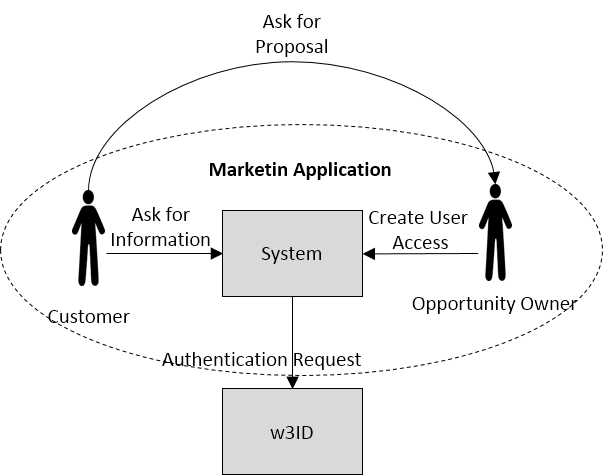
\includegraphics[width=\textwidth]{img/diagrams/Context.png}
    \caption[Application System Context Diagram]{Application System Context Diagram (own illustration)}
    \label{fig:my_label}
\end{figure}

In order to define the system context, the information collected in the previous section will be analyzed for implications on the four facets explained in \Cref{beginFacets} on \cpagerefrange{beginFacets}{endFacet}.

\subsection{Entities}
The main entity identified - to this point - to be identified is information about IBM knowledge and experience on banking software migration (mentioned in \textbf{I1, I7, I9 - I10} and most personas). This entity is core to the intend of most direct stakeholders and many expectations are related to those. Different customer employees demand different kinds of information, while all require the information to not be high level marketing formulations.

\paragraph{} Other entities relate to authentication: IBM employees must be represented in the system, in order to identify them when logging in (cf. \textbf{I4}). On the other hand customers must be reflected in the system. Those information must be related to authentication (cf. \textbf{I2}) and to the customer's individual business case (cf. \textbf{I7}. 
\subsection{IT-System}
The system must be able to connect to OAuth 2.0 services, as of demanded in \textbf{I4.2}.

\paragraph{} The system itself must run on a Bluemix Server (cf. \textbf{I13}), which can either be a Node.JS or a Java for Liberty (Java EE; cf. \cite{}). 

\subsection{Usage}
The users of the system are customer employees, IBM opportunity owner and the sponsor. An additional actor on the system is the developer. 

\paragraph{} Extracting from the personas of the customer employees, one can deuce that they want to have specific solutions for their defined problems. This follows the line of the subsection \say{B2B versus B2C Marketing}. There \textcite[21]{Backhaus.2015b} suggested that larger decision maker groups with defined requirements demand a individualized communication, as they are a custom to by sales men and proposal presentations. 

\paragraph{} As a basis to fulfill this goal, the sponsor demanded a UI and navigation based on common mobile banking apps. He also impied a access granting system for customers and IBM enforces a w3ID log in for IBM employees.

\paragraph{}
The complete use case diagram as it will be developed in the following is shown in \Cref{fig:ucucuc}:
\paragraph{}
\begin{figure}[H]
    \centering
    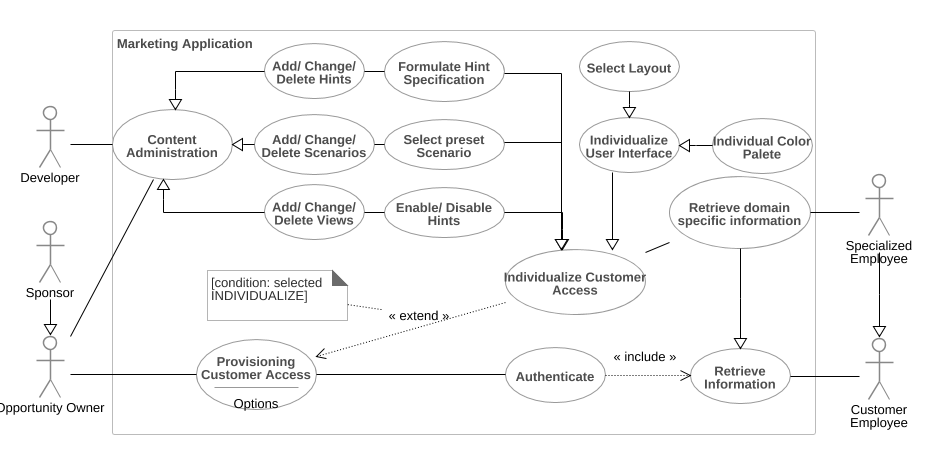
\includegraphics[width=\textwidth]{img/diagrams/UseCase.png}
    \caption[Use Case of the Application]{Use Case of the Application (own illustration)}
    \label{fig:ucucuc}
\end{figure}


\subsection{Development}
Different requirements regard the development of the application: 
\paragraph{}
\begin{itemize}
    \item Build on Bluemix
    \item Use an iterative approach.
\end{itemize}

\section{Engineering Requirements}

\begin{figure}[H]
    \centering
    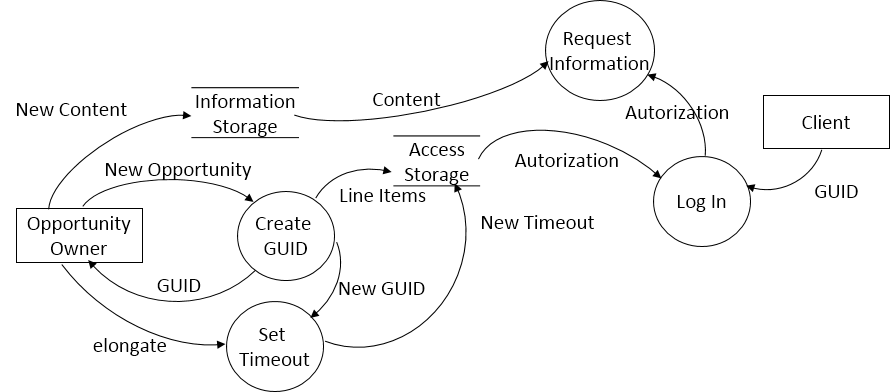
\includegraphics[width=\textwidth]{img/diagrams/FunctionDiagram.png}
    \caption[Functional Diagram of Application]{Functional Diagram of Application (own illustration)}
    \label{fig:}
\end{figure}

\paragraph{}
As by the sources described on the last pages, one can build a basic set of navigational requirements:
\paragraph{}
\begin{closeItem}
    \item [\textbf{FR1.1}] If a user clicks on a navigation element, the application shall be able to display the linked view.
    \item [\textbf{FR1.2}] If a user clicks on an element, the application shall be able to identify the clicked element.
    \item [\textbf{FR1.3}] When an element gets identified, the application shall be able to display the linked hint.
    \item [\textbf{FR1.4}] If a hint is displayed, the application shall provide the user the opportunity to hide the hint.
    \item [\textbf{FR1.4}] During usage, the application shall provide the user the a display of his progress (how many hint were displayed, how many to go)?.
    \item [\textbf{FR1.5}] When not in use, the application should save the progress of the user.
\end{closeItem}

\paragraph{}
Regarding the question of authentication of the customer employees. Registering every single one via e-mail would expensive in time, and as described earlier, time wasted paying attention on non productive work implies a direct cost of opportunity. The optimal way for a authentication process to work, would be a one click solution. This may be achieved by generating a random key per user, which can either be entered manually at the clients computer, or directly accessed by adding the code to the URL of the web page. This would enable the opportunity owner a fast quick solution, which will not be time intensive for the customer as well. As an example, the code may be passed e-mail, qr-code. The randomly generated number could be chosen arbitrary, this paper will use Global Unique Identifier (GUID). The process can also be seen in \Cref{fig:functionalaccess}
\begin{closeItem}
    \item [\textbf{FR2.1}] If the application website is accessed, the application shall provide administrators with the option to log in via w3ID.
    \item [\textbf{FR2.2}] When a administrator is logged in, the application shall provide the option to appoint new administrators (constraint: only IBM employees may be administrators).
    \item [\textbf{FR2.3}] When a administrator is logged in, the application shall provide the option to generate a new user access.
    \item [\textbf{FR2.4}] When a new user access is generated, the application shall generate a GUID-Token as identifier.
    \item [\textbf{FR2.5}] If the application website is accessed, the application shall provide users with the option to log in via GUID-Token.
    \item [\textbf{FR2.6}] After a two week time, if the token did not get elongated, the application shall ban the token from access.
\end{closeItem}

\begin{figure}[H]
    \centering
    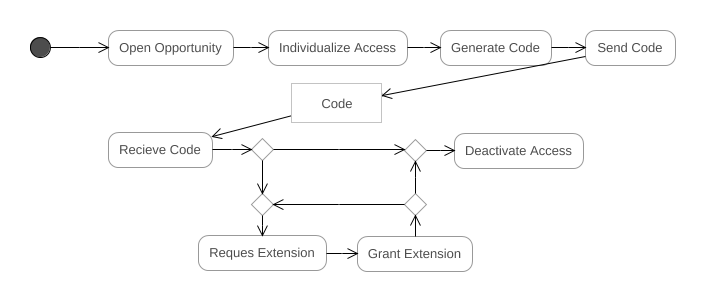
\includegraphics[width=\textwidth]{img/diagrams/Activity/AccessGranting.png}
    \caption[Access Granting Process]{Access Granting Process (own illustration)}
    \label{fig:functionalaccess}
\end{figure}

\paragraph{} A major demand by the personas is, to receive relevant information. Therefore, the content of the application must be updated whenever new major lessons learned occur. For this to be possible, first a content management for the application must be implemented:

\begin{closeItem}
    \item [\textbf{FR3.1}] When a administrator is logged in, the application shall provide the option to create, edit and delete hints.
    \item [\textbf{FR3.2}] When a administrator is logged in, the application shall provide the option to associate hints with elements from the user view.
    \item [\textbf{FR3.3}] When a administrator is logged in, the application shall provide the option to edit the structure of the user view.
\end{closeItem}

\paragraph{} The other major of the personas demand were individualized information and appearance. First, the individualized content: this cannot go to the cost of the opportunity owners time, if certain modifications are done repeatedly. In correspondence with the sponsor, three major scenarios were identified. For the requirements the specific scenarios are not relevant, but it is important do define what scenario in this context means: A template for a business case, commonly occurring (like a change in software), which requires some special formulations for some hints, and does not include others at all over the other cases. The same is true the other way around. 

\begin{closeItem}
    \item [\textbf{FR4.1}] When a administrator is logged in, the application shall provide the option to create to create  scenario.
    \item [\textbf{FR4.1}] When a scenario is created, the application shall provide administrators the option specify the content of hints and notifications.
     \item [\textbf{FR4.1}] When a administrator is logged in, the application shall provide the option to associate users and scenarios.
\end{closeItem}

\paragraph{} Secondly the first step towards individualization in user experience.Changing the color palette to the colors of the customer does not change the value of the software, but follows a much more accustomed view for the customer.

\begin{closeItem}
     \item [\textbf{FR5}] When a administrator is logged in, the application shall provide the option to change the color palette used per user.
\end{closeItem}

\paragraph{} In a later stage, also the ability to provide different layouts is interesting. This could also be a tool to keep the software uo to date, in terms of design. 

\begin{closeItem}
      \item [\textbf{FR6.1}] When a administrator is logged in, the application shall provide the option to upload new layouts in form of a CSS file to the server.
     \item [\textbf{FR6.2}] When a administrator is logged in, the application shall provide the option change the layout used per user.
\end{closeItem}

\paragraph{} Last, but not leas: The customer's stakeholders. At least the BaFin, being most influential in the stakeholder map, must be considered. The challenge is: the requirement of using a front office presentation as example, hinders the possibility to explain backoffice topics. Notifications can be used for that, in case they are supported by the device, the attention of a user can be retrieved by this technique. If not, the information can be displayed in kind of a fake notification. Additionally, the sponsor suggested a kind of offline availability for the application.

\begin{closeItem}
      \item [\textbf{FR7.1}] When not in foreground, the application should send notifications to the user.
      \item [\textbf{FR7.2}] When a administrator is logged in, the application should provide the option to create, edit and delete notifications, assign them to scenarios and formulate specifications for scenarios.
      \item [\textbf{FR7.3}] When connected to the internet, the user device should download the page contents for offline availability.
      
\end{closeItem}

The quality requirements are a selection from the Development guidelines of the \textcite{IBMCorporation.2016}. \textbf{QR1.5} is required for \textbf{QR1.4} to work.

\begin{closeItem}
      \item [\textbf{QR1.1}] When developing, the developer shall use automated testing, as described in \Cref{fig:test}.
      \item [\textbf{QR1.2}] When developing, the developer shall write the test cases before developing the module.
      \item [\textbf{QR1.3}] When developing, the developer shall focus on smart phones (iOS and Android) first.
      \item [\textbf{QR1.4}] When developing, the developer shall utilize a continuous delivery stream on the Bluemix platform. \item [\textbf{QR1.5}] Whenever new functionality is deployed, the application shall use default parameters in a way that it has no impact on current users.
      \item [\textbf{C1.1}] When developing, the developer shall use IBM Bluemix Git for version control.
\end{closeItem}

Testing is required by the \textcite{IBMCorporation.2016}. The actual test procedure (cf. \Cref{fig:test}) is based on the recommendation of \textcite{OpenWebApplicationSecurityProject.} and the requirements of the IBM Corporation. The first two steps ensure, that the application does what it is suppose to be. The following steps test the code quality and the server configuration, which ensures the page to firstly, appearing conscientiously developed, and secondly reducing the risk of being marked as an insecure web page by any browser.

\begin{figure}[H]
    \centering
    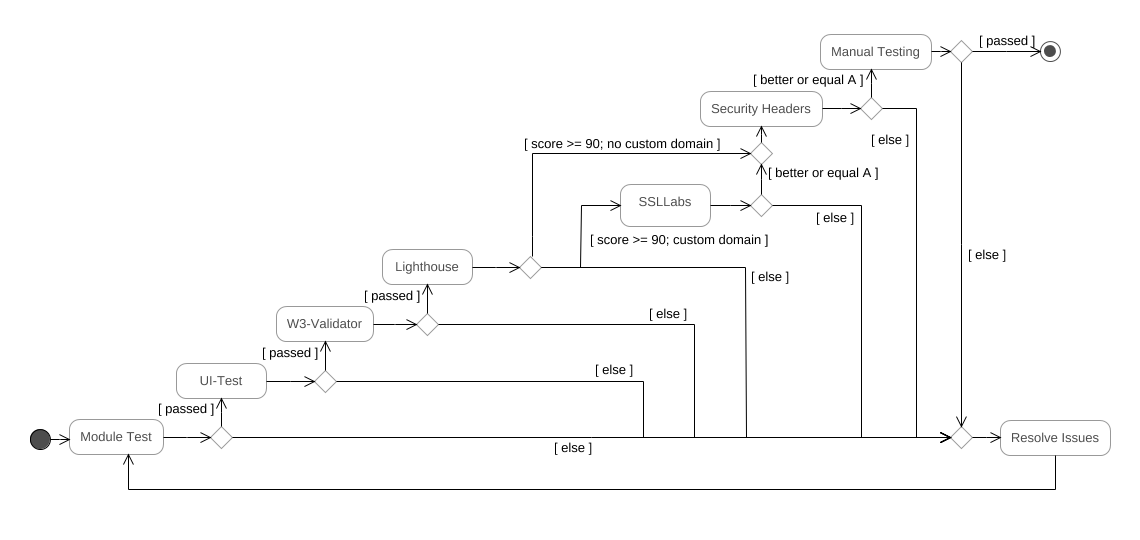
\includegraphics[width=\textwidth]{img/diagrams/Activity/Testing.png}
    \caption[Testing Procedure]{Testing Procedure (own illustration)}
    \label{fig:test}
\end{figure}


\subsubsection{Conception}

\begin{figure}[H]
    \centering
    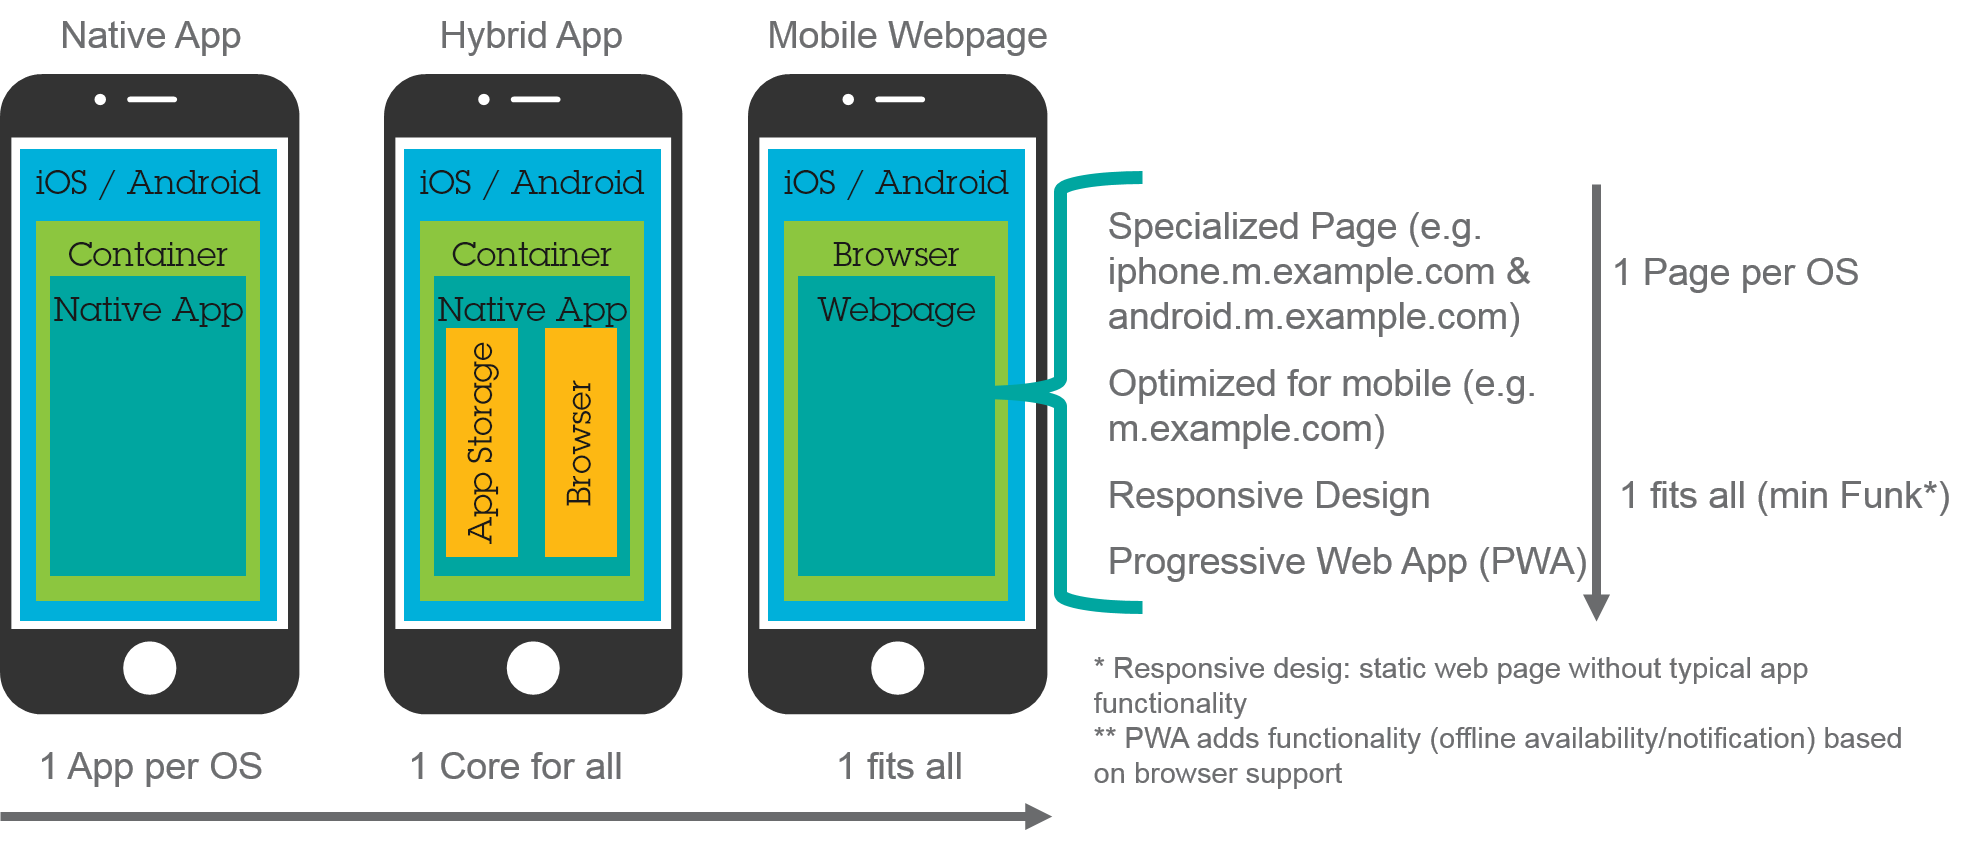
\includegraphics[width=\textwidth]{img/Alternatives.png}
    \caption[Responsive design alternatives]{Responsive design alternatives (own illustration)}
    \label{fig:}
\end{figure}

Conception of an application fulfilling the requirements above, requires an essential decision. Mobile devices must be addressed as it is required by the mobile first approach if nothing holds against it. In general three different basic designs of applications for - basically every computer but especially - mobile devices are possible:

\paragraph{} Firstly, one could write a native application. This would require the application to divide in basically one application per operating system. This would require much more effort than the second approach, which would be a hybrid solution. Hybrid apps are designed as a web page, but are contained in a native app wrapper. Thereby they can use most of the operating systems functionality, by having only one core application. On the other hand, the wrapper applications have to be maintained regularly \parencite[cf.][]{Vaiyapuri.25.05.2015}. 

\paragraph{} Last but not least, regular web pages can be received anywhere a internet connection is available, and for the central functionality of displaying information have no compatibility problems if done correctly. The point of doing it correctly heavily depends on the use case. It is possible to write one website per operating system, guaranteeing optimal comparability. On the other extreme, one does not even write a page per screen size, but does something called responsive design \parencite[cf.][]{Vaiyapuri.25.05.2015}. 

\paragraph{} While Responsively designed web pages have the least source code for serving the most devices, it has the least functionality. The JavaScript Standard is not implemented in every browser in the same version or at the same integrity \parencite[cf.][]{Zaytsev.2017}. This is countered by the progressive web app (PWA) idea. The PWA is a responsive web page, only using functionality which is supported everywhere, and add functionality as the browser supports it \parencite[cf.][]{GoogleDevelopers.}. As an example, if a browser supports sending the user notifications from the off, the website can implement this and send updates or news. Without this functionality the website still works, but just without notifications \parencite[cf.][]{Vaiyapuri.25.05.2015}. 

\paragraph{} Therefore, this paper suggest using PWAs when having low development resources and targeting a wide diversity of devices. This derives a new requirement:
\begin{closeItem}
      \item [QR1.5] May a feature not be available globally, the application must test the availability on the platform it is running first.
\end{closeItem}

\paragraph{} A quick list with suggestions for PWA features is added here, including fallback solutions if possible.
\begin{table}[H]
    \centering
    \begin{tabular}{m{5.33cm}|m{5.33cm}|m{5.33cm}}
    &   PWA-Technology &   Fallback    \\
    \hline 
Offline capability  &	ServiceWorkerCache   &   AppCache    \\
    \hline 
User Data Storage (e.g. Progress)	&   LocalStorage    &   Cookies    \\
    \hline 
User Interaction	&   Vibrate \& Notification  & ~~~  \\
    \end{tabular}
    \caption[Progressive Web App Features for the Case]{Progressive Web App Features for the Case (own illustration)}
    \label{tab:my_label}
\end{table}


\paragraph{} The backend decision gets a little easier through the decision for a PWA. Programmatic logic is added to web pages by using javascript. The two backend systems use java, respectively javascript as programming language. Having limited programming resources, and already using javascript, this paper decides on NodeJS, the javascript solution. This may not be universal, but the backend of this system must only deliver data to the client and read and write to and from a database. If the program would be more computing time intense, a comparison of performance may be useful, but not economic in this setting.
\begin{closeItem}
      \item [\textbf{C1.2}] When deploying, the application shall be deployed to a NodeJS Bluemix Service.
\end{closeItem}
\subsubsection{Visual Design}
Taking the conceptual approach suggested above, an visual design was built, based on the rules of the minimal design approach and the gestalt theory. The design of the application started of by analyzing different banking applications, which can be seen in the appendix. Based on those a structure was developed and was broken down into screens. After designing a general layout, the individual pages were filled in. The wire frames may be seen below with a brief explanation. 
\begin{figure}[H]
    \centering
    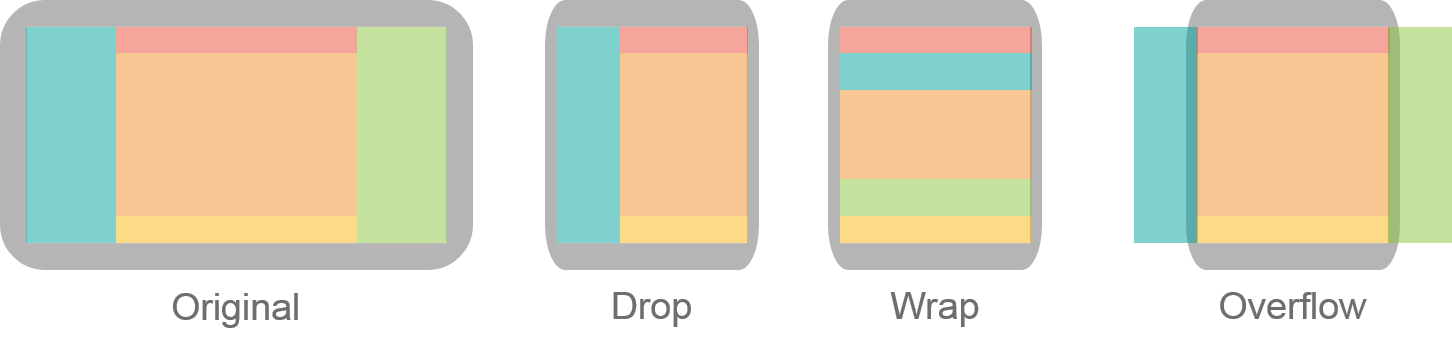
\includegraphics[width=\textwidth]{img/responsive.png}
    \caption[Responsive design alternatives]{Responsive design alternatives (own illustration)}
    \label{fig:response}
\end{figure}
Responsive design, being the foundation of PWAs, are designs, which change based on screen size, rather than being statically or fluit. Therefore it uses the techniques displayed in \Cref{fig:response}. Elements can be treated differently based on their importance and the overall design. As an example, right handed widget bars displaying information that can be read elsewhere as well, sometimes get dropped on smaller screens. On the other hand, menus are of such importance, that they either wrap, or flow outside the screen and can be retrieved by clicking on a button or something similar.
\begin{figure}[H]
    \centering
    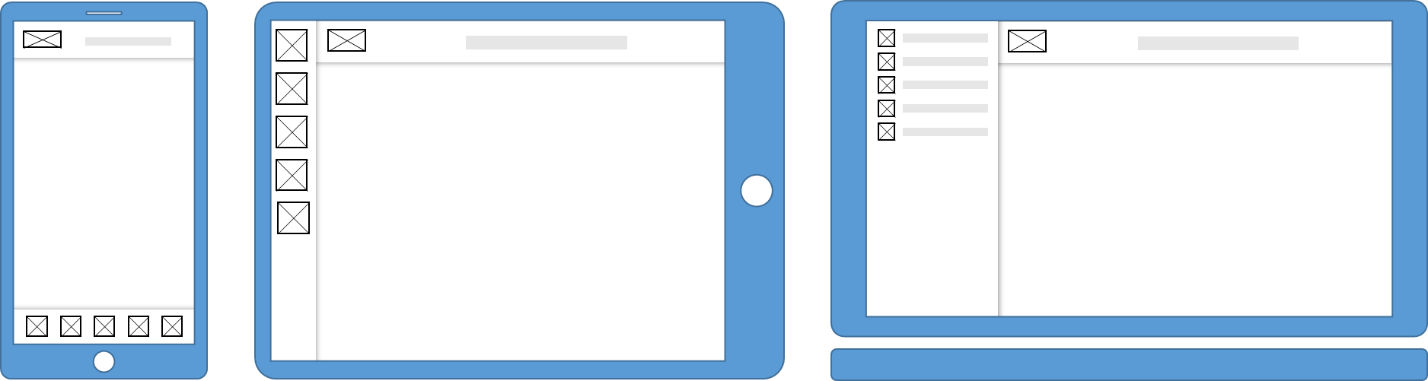
\includegraphics[width=\textwidth]{img/diagrams/wireframes/general.png}
    \caption[General Layout - Wireframe]{General Layout - Wireframe (own illustration)}
    \label{fig:}
\end{figure}
The general design of the application consists of a navigation bar, a title bar and a content area. The title bar fulfills no functionality, and may be drooped as of the suggestion by the minimal design approach. On the other hand prior knowledge of most applications suggest that those commonly have title bars. Therefore this design will use one in the first instance, but it may be removed as the development progresses. The menu bar follows the rules of responsive design, as it changes appearance depending on the screen size. Smart phone will have a bottom icon menu as it is known form Android and iOS home screens. On larger screens it wraps to the side and later displays the menu titles, which are dropped on smaller screens. The content area follows the responsive approach by wrapping across all screen sizes (see below).
\begin{figure}[H]
    \centering
    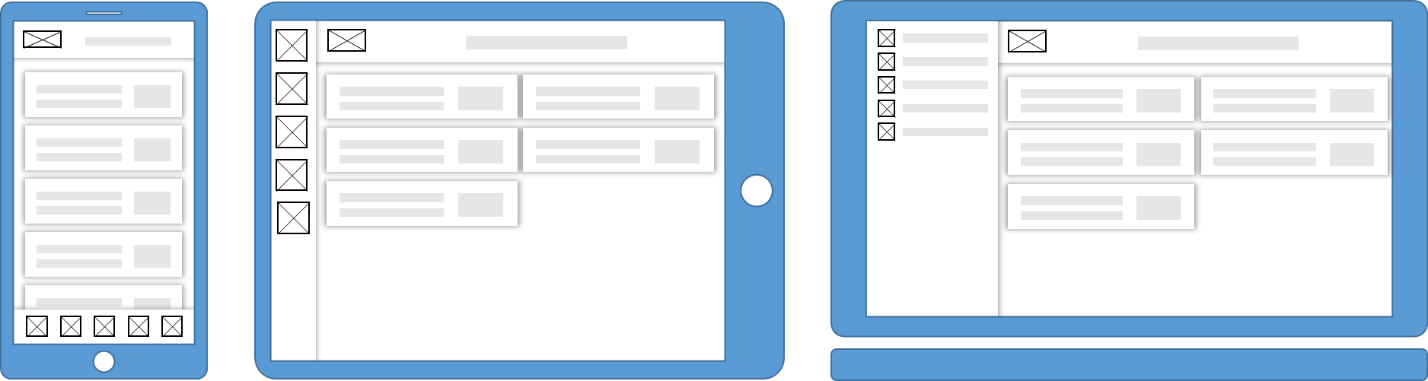
\includegraphics[width=\textwidth]{img/diagrams/wireframes/overview.png}
    \caption[Overview - Wireframe]{Overview - Wireframe (own illustration)}
    \label{fig:}
\end{figure}
Most elements in the prototype design are blocks. Those blocks can easily be grouped by common fate (scrolling while the general layout is fixed into position) and by proximity, while straight foreword separating the insides.
\begin{figure}[H]
    \centering
    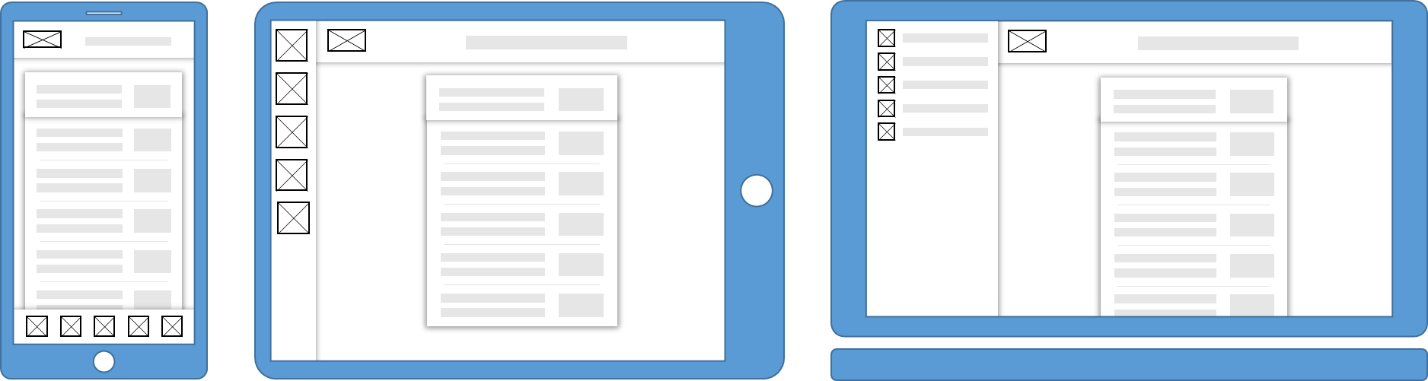
\includegraphics[width=\textwidth]{img/diagrams/wireframes/transaction.png}
    \caption[Transactions - Wireframe]{Transactions - Wireframe (own illustration)}
    \label{fig:}
\end{figure}
Transactions are grouped to the account by the law of good gestalt. This is achieved by continuing the block of the account. This view can be used for accounts and credits, but also for line items in a custody account.
\begin{figure}[H]
    \centering
    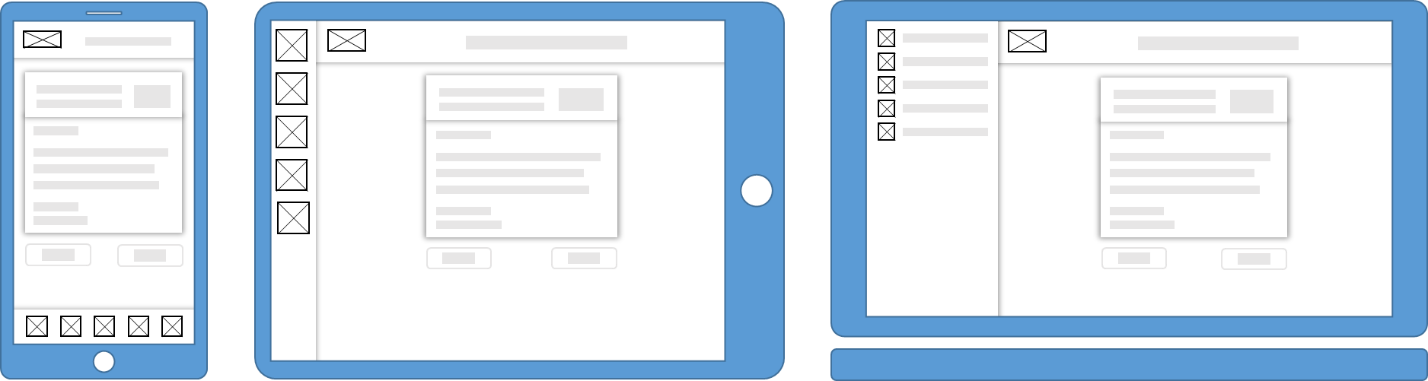
\includegraphics[width=\textwidth]{img/diagrams/wireframes/message.png}
    \caption[Message - Wireframe]{Message - Wireframe (own illustration)}
    \label{fig:}
\end{figure}
Messages are displayed as a single block, which has (if necessary) buttons beneath it. This can be useful when simulating e.g. new terms and conditions.
\begin{figure}[H]
    \centering
    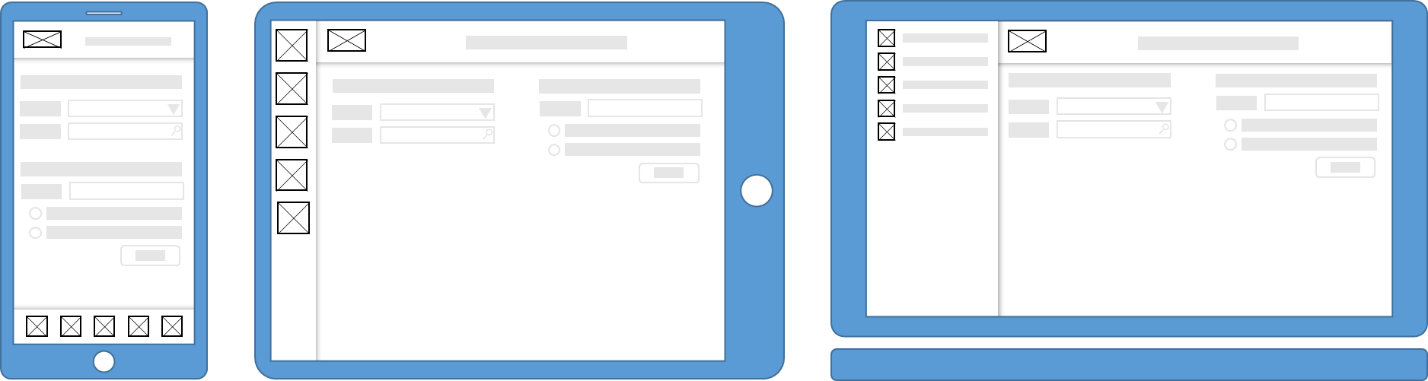
\includegraphics[width=\textwidth]{img/diagrams/wireframes/formular.png}
    \caption[Form - Wireframe]{Form - Wireframe (own illustration)}
    \label{fig:}
\end{figure}
Forms break out of the boxed design, because this would visually divide the elements of the form too strong. Grouping of form inputs belonging together will be achieved exploiting the law of proximity.
\begin{figure}[H]
    \centering
    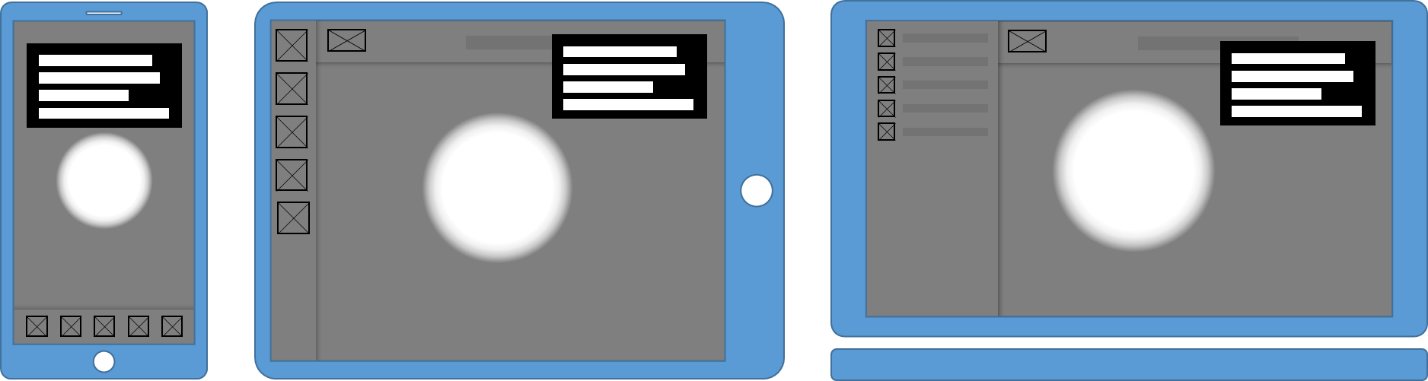
\includegraphics[width=\textwidth]{img/diagrams/wireframes/hint.png}
    \caption[Hint - Wireframe]{ - Wireframe (own illustration)}
    \label{fig:}
\end{figure}
\paragraph{}
Hints are displayed with an overlay. This removes other elements from the focus of the viewer and extracts the selected element from all groups it was integrated in before. This is achieved by a highlighting circle, besides which the hint content is displayed.
\begin{figure}[H]
    \centering
    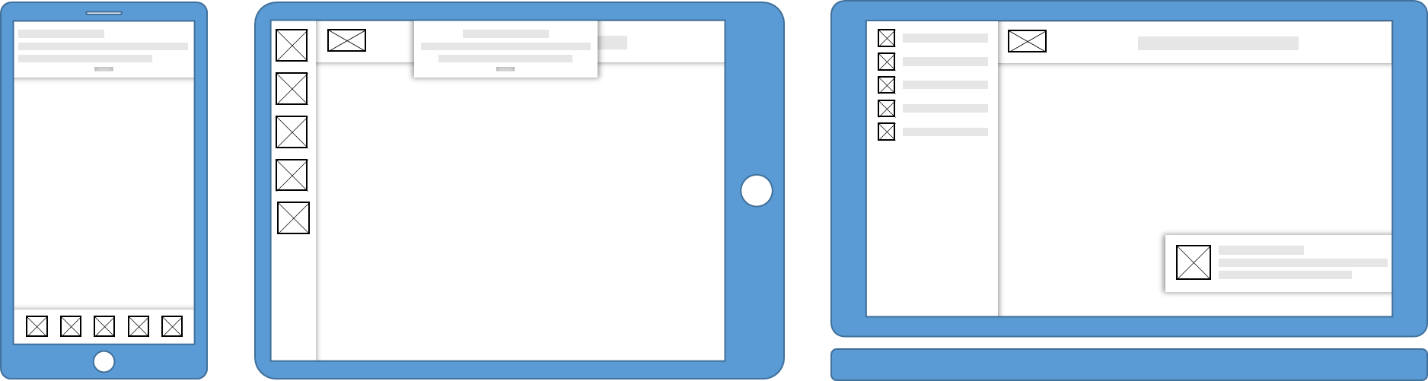
\includegraphics[width=\textwidth]{img/diagrams/wireframes/notification.png}
    \caption[Notification - Wireframe]{Notification - Wireframe (own illustration)}
    \label{fig:}
\end{figure}
\paragraph{}
Notifications, as mentioned in \textbf{FR7.2}, are done in a fashion as they are commonly know at the corresponding devices, thereby using prior knowledge as suggested by the minimal design approach. These may be either achieved by using the devices Notification API, or otherwise simulate a similar experience by building them in the page with HTML and JS, as the PWA principle suggests.
\chapter{Discussion}
The requirements and basic conception done in this paper shows exemplary, how a B2B marketing app may be concepted. It is to say, that relatively few conceptual aspects can be found. The only set of requirements directly substituted from the specialties of B2B marketing, are the requirements regarding narrower approach of the individual case, as it would be possible in a B2C environment. 

\paragraph{} More directly can be drawn from this paper, that the approach on information sourcing needs to be adjusted to this setting. The sources for this paper were nearly exclusively from inside IBM, when regarding the personas. Qualitative research was close to impossible, because the stakeholders were fully involved in projects and had no time for interviews. Also Quantitative research would have exceeded the scope of this paper. Further research in this direction needs to be done for concluding results. 

\paragraph{} It is important to note, that the approach of regarding the customer's stakeholder gave good insight, but will have more effect on the contents of the application than on the concept. 

\chapter{Conclusion}
This paper found no satisfying set of aspects to consider when designing an B2B marketing app. Only two core aspects were identified:

\begin{itemize}
\item B2B marking apps require a high flexibility in content in order to fit the specific business case.
\item It could be verified that an investigation along the supply chain down to the consumer can give important insights to be considered when designing the app.
\end{itemize}

\paragraph{} Because this paper could not find a diverse set of information on the customer, thereby these results can at most be regarded as hypothesis. Further research will have to show whether these conclusions will be confirmed.
